%---------- Inleiding ---------------------------------------------------------

\section{Introductie} % The \section*{} command stops section numbering
\label{sec:introductie}

Machine learning en eenvoudig in dezelfde zin gebruiken, geen vanzelfsprekende opdracht maar wel iets dat Google probeert te realiseren. Met eigenschappen op hun site \autocite{Google2019} zoals: Uitstekende prestaties; Snel aan de slag; ontstaan er met Cloud AutoML toch enkele mogelijkheden om als programmeur (zonder professionele AI kennis) machine learning diensten te voorzien in een applicatie zonder dat er een data scientist bij het project betrokken wordt. Dit onderzoek, gefocust op het classificeren en herkennen van afbeeldingen, probeert aan te tonen dat deze service bruikbaar is voor bedrijven en hoe het scoort tegenover alternatieven.

%---------- Stand van zaken ---------------------------------------------------

\section{Literatuurstudie}
\label{sec:literatuurstudie}

% Voor literatuurverwijzingen zijn er twee belangrijke commando's:
% \autocite{KEY} => (Auteur, jaartal) Gebruik dit als de naam van de auteur
%   geen onderdeel is van de zin.
% \textcite{KEY} => Auteur (jaartal)  Gebruik dit als de auteursnaam wel een
%   functie heeft in de zin (bv. ``Uit onderzoek door Doll & Hill (1954) bleek
%   ...'')

Geautomatiseerde machine learning is het automatiseren van het trainingsproces bij een artificieel neuraal netwerk. De lage toegangsdrempel zorgt ervoor dat mensen met beperkte machine learning kennis sneller en simpeler een model kunnen trainen en gebruiken.

\subsection{Natural Architecture Search}

\begin{figure}
    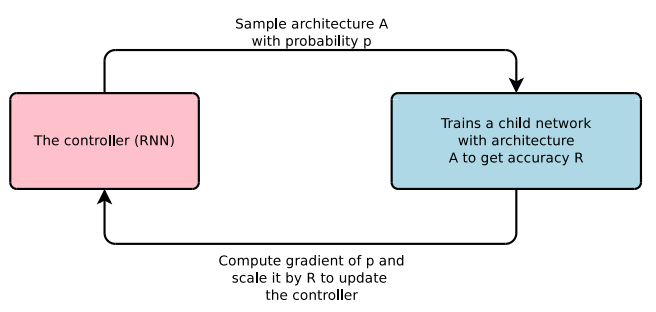
\includegraphics[width=\linewidth]{img/nas.png}
    \caption{Werking van Neural Architecture Search}
    \label{fig:nas}
\end{figure}

Dergelijke AutoML systemen gebruiken een techniek die het ontwerp van een artificieel neuraal netwerk kan automatiseren, beter bekend als Natural Architecture Search \autocite{Elsken2019}. Uit \textcite{ZophL2016} wordt vastgesteld dat deze techniek een gelijkaardige of zelfs betere performantie heeft dan modellen die door een ML-ingenieur ontworpen zijn.

Natural Architecture Search gebruikt Reinforcement Learning om een model te trainen. Deze manier van werken is fundamenteel anders dan gesuperviseerd / ongesuperviseerd leren omdat het model niet beter wordt door het gebruik van datasets. Als alternatief kan het neuraal netwerk beloningssignalen herkennen waardoor het kan leren welke acties leiden tot een positief resultaat \autocite{Lievens2019}.

Op figuur \ref{fig:nas} wordt gevisualiseerd hoe dit werkt. Op basis van controller structuur A (waarbij A een neuraal netwerk is) wordt een string met variabele lengte gegenereerd. Deze waarden worden gebruikt als parameters om een kind-netwerk aan te maken, die getraind wordt met echte data en waarbij de accuraatheid gemeten wordt aan de hand van een validatie dataset. Het resultaat wordt gebruikt als beloningssignaal voor de controller, bij de volgende iteratie kunnen er hogere kansen gegeven worden aan parameters die leiden tot accurate voorspellingen \autocite{ZophL2016}. De controller zijn zoekfunctie zal dus verbeteren over tijd.

\subsection{Hyperparameter tuning}

In de vorige sectie is het gebruik van parameters aan bod gekomen. Ze bepalen het gedrag van een neuraal netwerk en zijn bepalend voor het eindresultaat. Volgens \textcite{Brust2019} zijn verschillende manieren om dit te behandelen. Brute force zal elke configuratie overlopen en beslissen hoe het model vordert terwijl feature selection gewichten aan verschillende parameters geeft. Op die manier hebben vorige simulaties een impact bij de selectie van een nieuwe set parameters \autocite{Claesen2015}.

\subsection{AutoML platformen}

Eerder is Google Cloud AutoML al aan bod gekomen. De familiaire interface helpt een gebruiker snel op weg. Naast Google hebben bedrijven zoals Microsoft en Amazon een platform gebouwd op hun respectievelijke cloud infrastructuur. De AutoML service kan voordelig zijn als het bedrijf al verwerkt zit in de stack, extra kosten kunnen snel de lucht in gaan zonder toegang tot andere functies (bv. van Google Cloud) als dit niet het geval is. Een open source alternatief lijkt een goede oplossing, de interfaces zijn minder gebruiksvriendelijk dan een betalend product en er komt meer programmeerwerk aan te pas. Het resultaat is vaak commercieel bruikbaar zolang de restricties van de licentie gerespecteerd worden \autocite{Balter2015}. AutoKeras is een voorbeeld onder de MIT licentie, die geen commerciële restricties oplegt.

%---------- Methodologie ------------------------------------------------------
\section{Methodologie}
\label{sec:methodologie}

Eerst en vooral wordt er een image dataset gemaakt die gebruikt wordt om de modellen te trainen en te valideren. Om een model te trainen is er een grote hoeveelheid data nodig. FFmpeg is een tool waarmee je de frames van een video (in dit geval een 360 graden video van het object) kan opsplitsen in afbeeldingen. De classificatie van de images wordt verwerkt met pandas, een data-analyse library voor Python.

Voor het experiment worden 2 modellen getraind met Google Cloud AutoML en AutoKeras. Zo kan het resultaat vergeleken worden met een open source alternatief. 

Er worden een aantal afbeeldingen geselecteerd van verschillende moeilijkheidsgraden om de modellen te toetsen.

%---------- Verwachte resultaten ----------------------------------------------
\section{Verwachte resultaten}
\label{sec:verwachte_resultaten}

\begin{figure}
    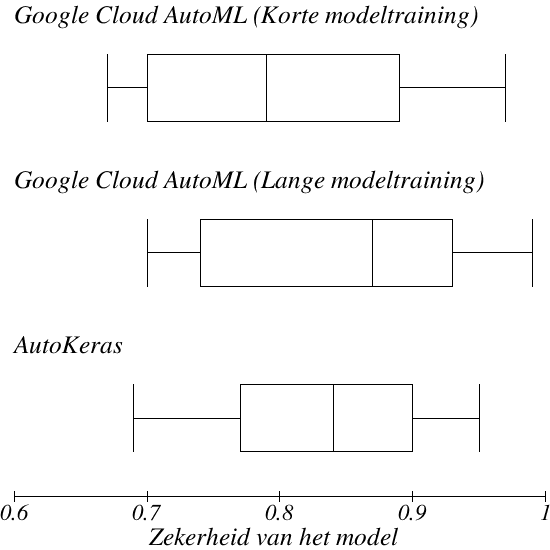
\includegraphics[width=\linewidth]{img/boxplot.png}
    \vspace{1mm}
    \caption{Verwachte correctheid van de modellen}
    \label{fig:boxplot1}
\end{figure}

Er worden goede resultaten verwacht van Google Cloud AutoML. Je betaalt voor een service en dan wil de gebruiker positieve resultaten op tafel zien. De trainingsduur van het Google Cloud AutoML model zal ook een zichtbare en positieve impact hebben op de gemiddelde score van een afbeelding. Uit het verleden hebben we geleerd dat \emph{community driven development} vaak leidt tot een performant resultaat (bv. de niet automatische versie, Keras) dat door veel developers onderhouden wordt. Voor een bedrijf is dit zeer interessant vanwege het kostenplaatje dat volledig wegvalt voor het gebruik van de technologie. 

Figuur \ref{fig:boxplot1} bevat een voorspelling van de prestaties voor de verschillende modellen.

%---------- Verwachte conclusies ----------------------------------------------
\section{Verwachte conclusies}
\label{sec:verwachte_conclusies}

AutoML zal zeker zijn plaats houden binnen het domein van machine learning. De Google Cloud AutoML interface zorgt voor een gebruiksvriendelijke omgeving waar zeer weinig programmatie aan te pas komt. Met AutoKeras moet de gebruiker meer kennis hebben van Python libraries (pandas, numpy, keras...) om hetzelfde resultaat te verkrijgen. 

Voor bedrijven lijkt het interessanter om voor open source te kiezen als het overeen komt met hun identiteit. Zo kunnen developers een kleine machine learning implementatie voorzien terwijl een data scientist zich kan bezig houden in grotere projecten.

